\documentclass[letterpaper,twocolumn,10pt]{article}
\usepackage{graphicx, url, epsfig, dirtree, hyperref, relsize}

\title{CprE 4870 Hardware Design for Machine Learning Term Project: Framework Comparison and Exploration}
\author{
{\rm Henry Shires}\\
hcshires@iastate.edu\\
Iowa State University
\and
{\rm Anthony Manschula}\\
tonyman2@iastate.edu\\
Iowa State University
\and
{\rm Alexander Bashara}\\
abashara@iastate.edu\\
Iowa State University
}
\date{Fall 2024}

\begin{document}

\maketitle

\section{Project Aims and Motivation}

Due to high demand in the fields of computer engineering and artificial intelligence, the tech industry is searching for faster ways to train, test, and deploy models. Given the recent explosion in popularity of powerful large language and generative machine learning models, it seems reasonable to assume that more and more people will want to get into using and customizing machine learning models for their own purposes. An important consideration is that these individuals may not have an extensive amount of ML background, which makes a well-documented and easy-to-use framework a very beneficial asset.

In the past, TensorFlow has been the go-to for researchers. In the past five to six years, however, PyTorch has seen a massive uptick in research use \cite{oconnor}, indicating that PyTorch has been the preference for leading edge research activity. Coupled with the fact that in 2021, 92\% of the models available on HuggingFace.co were PyTorch exclusive \cite{oconnor}, it makes sense to make the move to a more widely used and supported framework. A distinguishing factor of PyTorch is that it uses dynamic computation graphs, whereas TensorFlow’s are static \cite{boesch}. While this offers more flexibility in terms of input data sizes, its dynamic nature means that it’s more difficult to optimize. PyTorch is typically regarded to be easier to work with due more closely following typical Python conventions.

Our team had no machine learning background before coming into this class and found lab 1 to be a bit of a steep introduction given TensorFlow’s relatively sparse documentation. Therefore, we have developed a redesign to lab 1 using PyTorch as opposed to TensorFlow. We have implemented the core learning points and activities of lab 1 using this new framework and have done analysis of the usability (in terms of documentation and relative difficulty of using the framework), training accuracy, and performance/resource utilization of PyTorch versus TensorFlow.

\section{Design Approach}
This project aims to allow us to draw various comparisons between the user experience, performance, and accuracy of the TensorFlow and PyTorch frameworks. We approached the design of the project in several steps, beginning with identifying the appropriate libraries, researching PyTorch equivalents of various TensorFlow functions, and code implementation. 

\subsection{Libraries}
The team identified several libraries we'd need to install to facilitate our research on PyTorch. These included the basic \verb|torch| and \verb|torchvision| plugins, as well as some utility libraries like \verb|matplotlib| and \verb|numpy|. However, in order to achieve the same functionality present in the TensorFlow approach, we needed to research additional libraries. As the \textit{TinyImageNet} dataset provided for Lab 1 was designed to be used with TensorFlow, we needed to find an equivalent for our PyTorch implementation. Our design utilizes the \verb|tinyimagenet| Python package, maintained by PyPI user \textit{facundoq}, which provides the dataset class and easily allows us to instantiate it. To provide detailed model summary reports, we opted to use the \verb|torch-summary| package, maintained by PyPI user \textit{tyleryep}. All other functionality of the TensorFlow Lab 1 was achievable using functions native to the core PyTorch package.

\subsection{PyTorch Equivalents}
As expected, PyTorch and TensorFlow differ in terms of semantics and API calls. Before we began writing code, we researched several areas that we believed would pose the most difficulty in porting to PyTorch.

The first area the group focused on pertained to model creation and training. For the most part, the layer naming was roughly the same as in TensorFlow, but this is about where the similarities end. Overall, in this regard, PyTorch is considerably more verbose in terms of syntax. Whereas TensorFlow allows the user to directly instantiate a Sequential model and add layers to it, PyTorch requires the user to define a new class that implements several functions in order to instantiate a model. Additionally, activation functions are not treated as part of a convolution or dense layer, but rather their own discrete layers, which posed some issues when exporting model weights. Below we provide an example of the code used to instantiate a model in PyTorch.
\begin{verbatim}
class TinyImageNetModel(nn.Module):
def __init__(self):
    super().__init__()
    self.tinyimgnet_model = nn.Sequential(
        nn.Conv2d(3, 32, (5, 5)),
        nn.ReLU(),
        ...
        nn.Linear(256, 200)
        nn.Softmax(dim=1)
    )

def forward(self, x):
    output = self.tinyimgnet_model(x)
    return output
\end{verbatim}
We can see that the model is defined within an init function within its own class. The layer setup looks very similar to what is seen in TensorFlow. However, one notable extra is that the user must also define their own forward propagation function, unlike in TensorFlow. This could potentially allow for more flexibility in model creation, however it also adds complexity that a new user may be less equipped to deal with.

Exploring the model training aspect, PyTorch strays even farther from TensorFlow in similarity. While TensorFlow provides an extremely convenient \verb|fit()| function that kicks off the training loop, PyTorch has no such equivalent and the training loop must be manually defined by the user. There are different ways of going about this, but PyTorch documentation recommends creating a function that trains the network on a per-epoch basis, which can then be wrapped in a separate loop to train for a desired number of epochs. We chose to implement a modified version of this approach for our project by adding a utility function to our TinyImageNetModel class for training purposes. We defined a \verb|_step()| function that would return loss and training accuracy for one batch of data:
\begin{verbatim}
def _step(self, step_name, batch):
    data, labels = batch
    f_loss = torch.nn.CrossEntropyLoss()

    # data/labels preloaded to device memory 
    # prior to training
    pred = self.forward(data).to(self.device)
    loss = f_loss(pred, labels).to(self.device)

    acc = Accuracy(task="multiclass", num_classes=200)
    acc_val = acc(pred.argmax(dim=1), labels)

    return (loss, acc_val)
\end{verbatim}
This function is called by another function (\verb|train_step()|) which essentially just supplies the \verb|step_name| variable, which is not shown here for brevity. The training loop calls the \verb|training_step()| function for each new batch of data that it pulls from the DataLoader and reports the loss and training set accuracy for each epoch. The core training loop consists of several distinct steps. First, we commence a transfer of model and full training image and label data to the compute device being used. We then zero the optimizer's gradients, call the step function (which calculates the loss), backpropagate the loss, and then execute the optimizer:
\begin{verbatim}
for epoch in range(epochs):
    for x, y in dataloader:
        loss, acc = model.train_step((x, y))
        epoch_loss += loss
        epoch_accuracy += acc
        opt.zero_grad()
        loss.backward()
        opt.step()
        i += 1
\end{verbatim}
Some informational printouts for average epoch loss and accuracy included in the full source code are not shown here.

Another area the team chose to look into was the method of tracing and profiling that we'd need to use. To perform inference profiling, TensorFlow works with Tensorboard for visualization. To use it, you must install the Tensorboard extension and start a server. The user can then import log files generated by the TF profiler during execution. The equivalent PyTorch implementation simply uses the built-in \verb|torch.profiler| library. We can wrap the inference call with a call to the profiler to gather execution time data on it:
\begin{verbatim}
act = [ProfilerActivity.CPU]
with profile(activities=act) as prof:
    with record_function("e2e_inference"):
        model(samples[0][0])
\end{verbatim}
We can then export this data to a json file using \verb|prof.export_chrome_trace(trace.json)|. The data can then be visualized using a variety of trace viewers, such as a web-based one like \textit{Perfetto UI}. Furthermore, we can also directly print execution time data to the console by calling \verb|prof.key_averages().table()|.

The last area that was slightly more complex compared to TensorFlow was the method in which datasets are loaded and used. In TensorFlow, the dataset is directly imported and used by the model. In PyTorch, it is possible to use the \verb|Dataset| object directly, but using a \verb|DataLoader| object to manage the dataset makes it much more straightforward to set batch sizes and shuffle them.

\subsection{Implementation}
In terms of implementation, we aimed to keep as many core learning points of the original lab as possible. This includes major areas like dataset exploration, learning how to perform inference on the data, accuracy calculations, model exploration and export, performance profiling, and model training and validation.

\section{Final Status}
Ultimately, the team accomplished all the objectives that we had planned to do in the proposal. Notably, due to the inclusion of an additional team member post-proposal submission, we have also decided to make an effort at delivering a modified Lab 1 document to further facilitate potential adoption of PyTorch as the machine learning framework of choice for future CPRE 487/587 classes.

\section{Results}

\subsection{Deliverable 1: PyTorch Jupyter Notebook and Benchmarks}
In order to comprehend the benefits and drawbacks between the two frameworks, we benchmarked PyTorch and TensorFlow in each of the following areas.

\subsubsection{Usability}
Here, we compare the ease of use of each frameworks' Python API, the clarity and usefulness of the documentation for each API, and the percentage of TensorFlow activities required in Lab 1 that could not be implemented in PyTorch.

While the metric "ease of use" is fairly subjective, there were a few areas where there were clear differences in the two frameworks, namely their associated documentation and conciseness of (most) code. Referencing the documentation is something that most people find themselves doing quite frequently unless they're intimately familiar with the particular tool they're using. Throughout the process of completing lab 1 for the first time and over the course of re-implementing it in PyTorch for this project, we made extensive use of each framework's documentation. In general, we can confidently say that the level of information and usability of the PyTorch documentation necessary to re-implement Lab 1 typically exceeds the that of the documentation we leveraged when initially completing Lab 1. For example, take the PyTorch~\cite{convtorch} and TensorFlow~\cite{convtensor} documentation pages for the 2D convolutional layer. The TensorFlow documentation has only a description of the arguments to the layer, some short details on input and output shape, object methods, and a short example. PyTorch, on the other hand, not only contains this information, but also provides details on what formulas and algorithms the layer is using to compute its output as well as several tips and notes to the user. Overall, this trend holds for a majority of the documentation pages that we referenced, and we believe the inclusion of this extra information contributes to PyTorch's accessibility to someone without a lot of machine learning experience.

We found the verbosity and clarity of the actual code implementation to be relatively similar. Most utility functions, such as \verb|.flatten()| and model loading, are present and used similarly across both frameworks. In the context of performance profiling, PyTorch wins out by a significant margin, not requiring the user to install any additional tools like Tensorboard to generate and view trace data. Gathering performance data is as simple as importing the Torch profile utility class. Generating a trace is then as simple as wrapping the desired chunk of code in a \verb|with| block and calling an export function:
\begin{verbatim}
with profile(activities=activities) as prof:
    with record_function("profiled_section"):
        [code-to-profile]
prof.export_chrome_trace("perf_trace.json")
\end{verbatim}
The trace can then be imported into a web-based tool like \textit{Perfetto UI}~\cite{perfetto} for viewing. An example is provided in \autoref{fig:perfetto}.
\begin{figure}[ht]
    \centering
    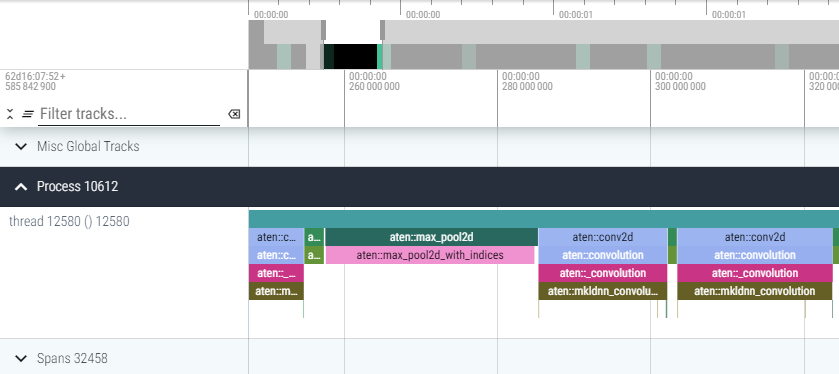
\includegraphics[width=1.07\linewidth]{Figures/perfetto.png}
    \caption{\textit{Excerpt of a Perfetto UI trace}}
    \label{fig:perfetto}
\end{figure}

However, PyTorch falls short of TensorFlow in a few areas, specifically exporting intermediate model activations and model training. To detach and visualize activations from intermediate layers of the model, TensorFlow simply requires the user to specify a variable in which to place them as an argument when constructing the model. For instance \verb|new_model = tf.keras.models.Model(inputs=|\\\verb|model.input, outputs=layer_outputs)| would place the activations as a list into the \verb|layer_outputs| variable. However, this process is considerably more verbose in PyTorch. The user must explicitly 'hook' each layer for which they want to view intermediate activations by detaching the output of the layer as follows:
\begin{verbatim}
activation = {}
def get_activation(name):
    def hook(model, input, output):
        activation[name] = output.detach()
    return hook
\end{verbatim}
The user must then call \verb|register_forward_hook(hook)| on each layer, when then makes each layer's activations available in the \verb|activation| list after running inference with the model. This process was not very straightforward and required a decent amount of research to figure out what was necessary to implement. 

Model training in PyTorch is significantly more involved than training in TensorFlow. TensorFlow just needs to user to call \verb|.fit()| and specify an input and number of epochs to begin training; PyTorch provides no such convenience. Our training code and associated utility functions total to approximately 75 lines, and required a large deal of research and experimentation to get working (discussed more in section 6.2). This area was certainly less user-friendly than TensorFlow.

Also, as noted in our initial proposal, we promised to record any core points assessed in lab 1 that were not possible to implement with PyTorch as opposed to TensorFlow. After implementing our PyTorch notebook, we were successfully able to complete all core points and had no need to skip any, further justifying the usability of PyTorch given this lab's application.

\subsubsection{Training Accuracy}
We compared PyTorch's ability to train high quality models. We trained the toy CNN model provided in Lab 1 on PyTorch using a different number of epochs and batch sizes as they were specified in the TensorFlow lab.

The overall accuracy of both frameworks after training the models through the different batch sizes at a fixed 20 epochs was relatively comparable, within about 10\% of each other. \autoref{fig:batchacc} shows a chart comparing the accuracy across different batch sizes.

\begin{figure}[ht]
    \centering
    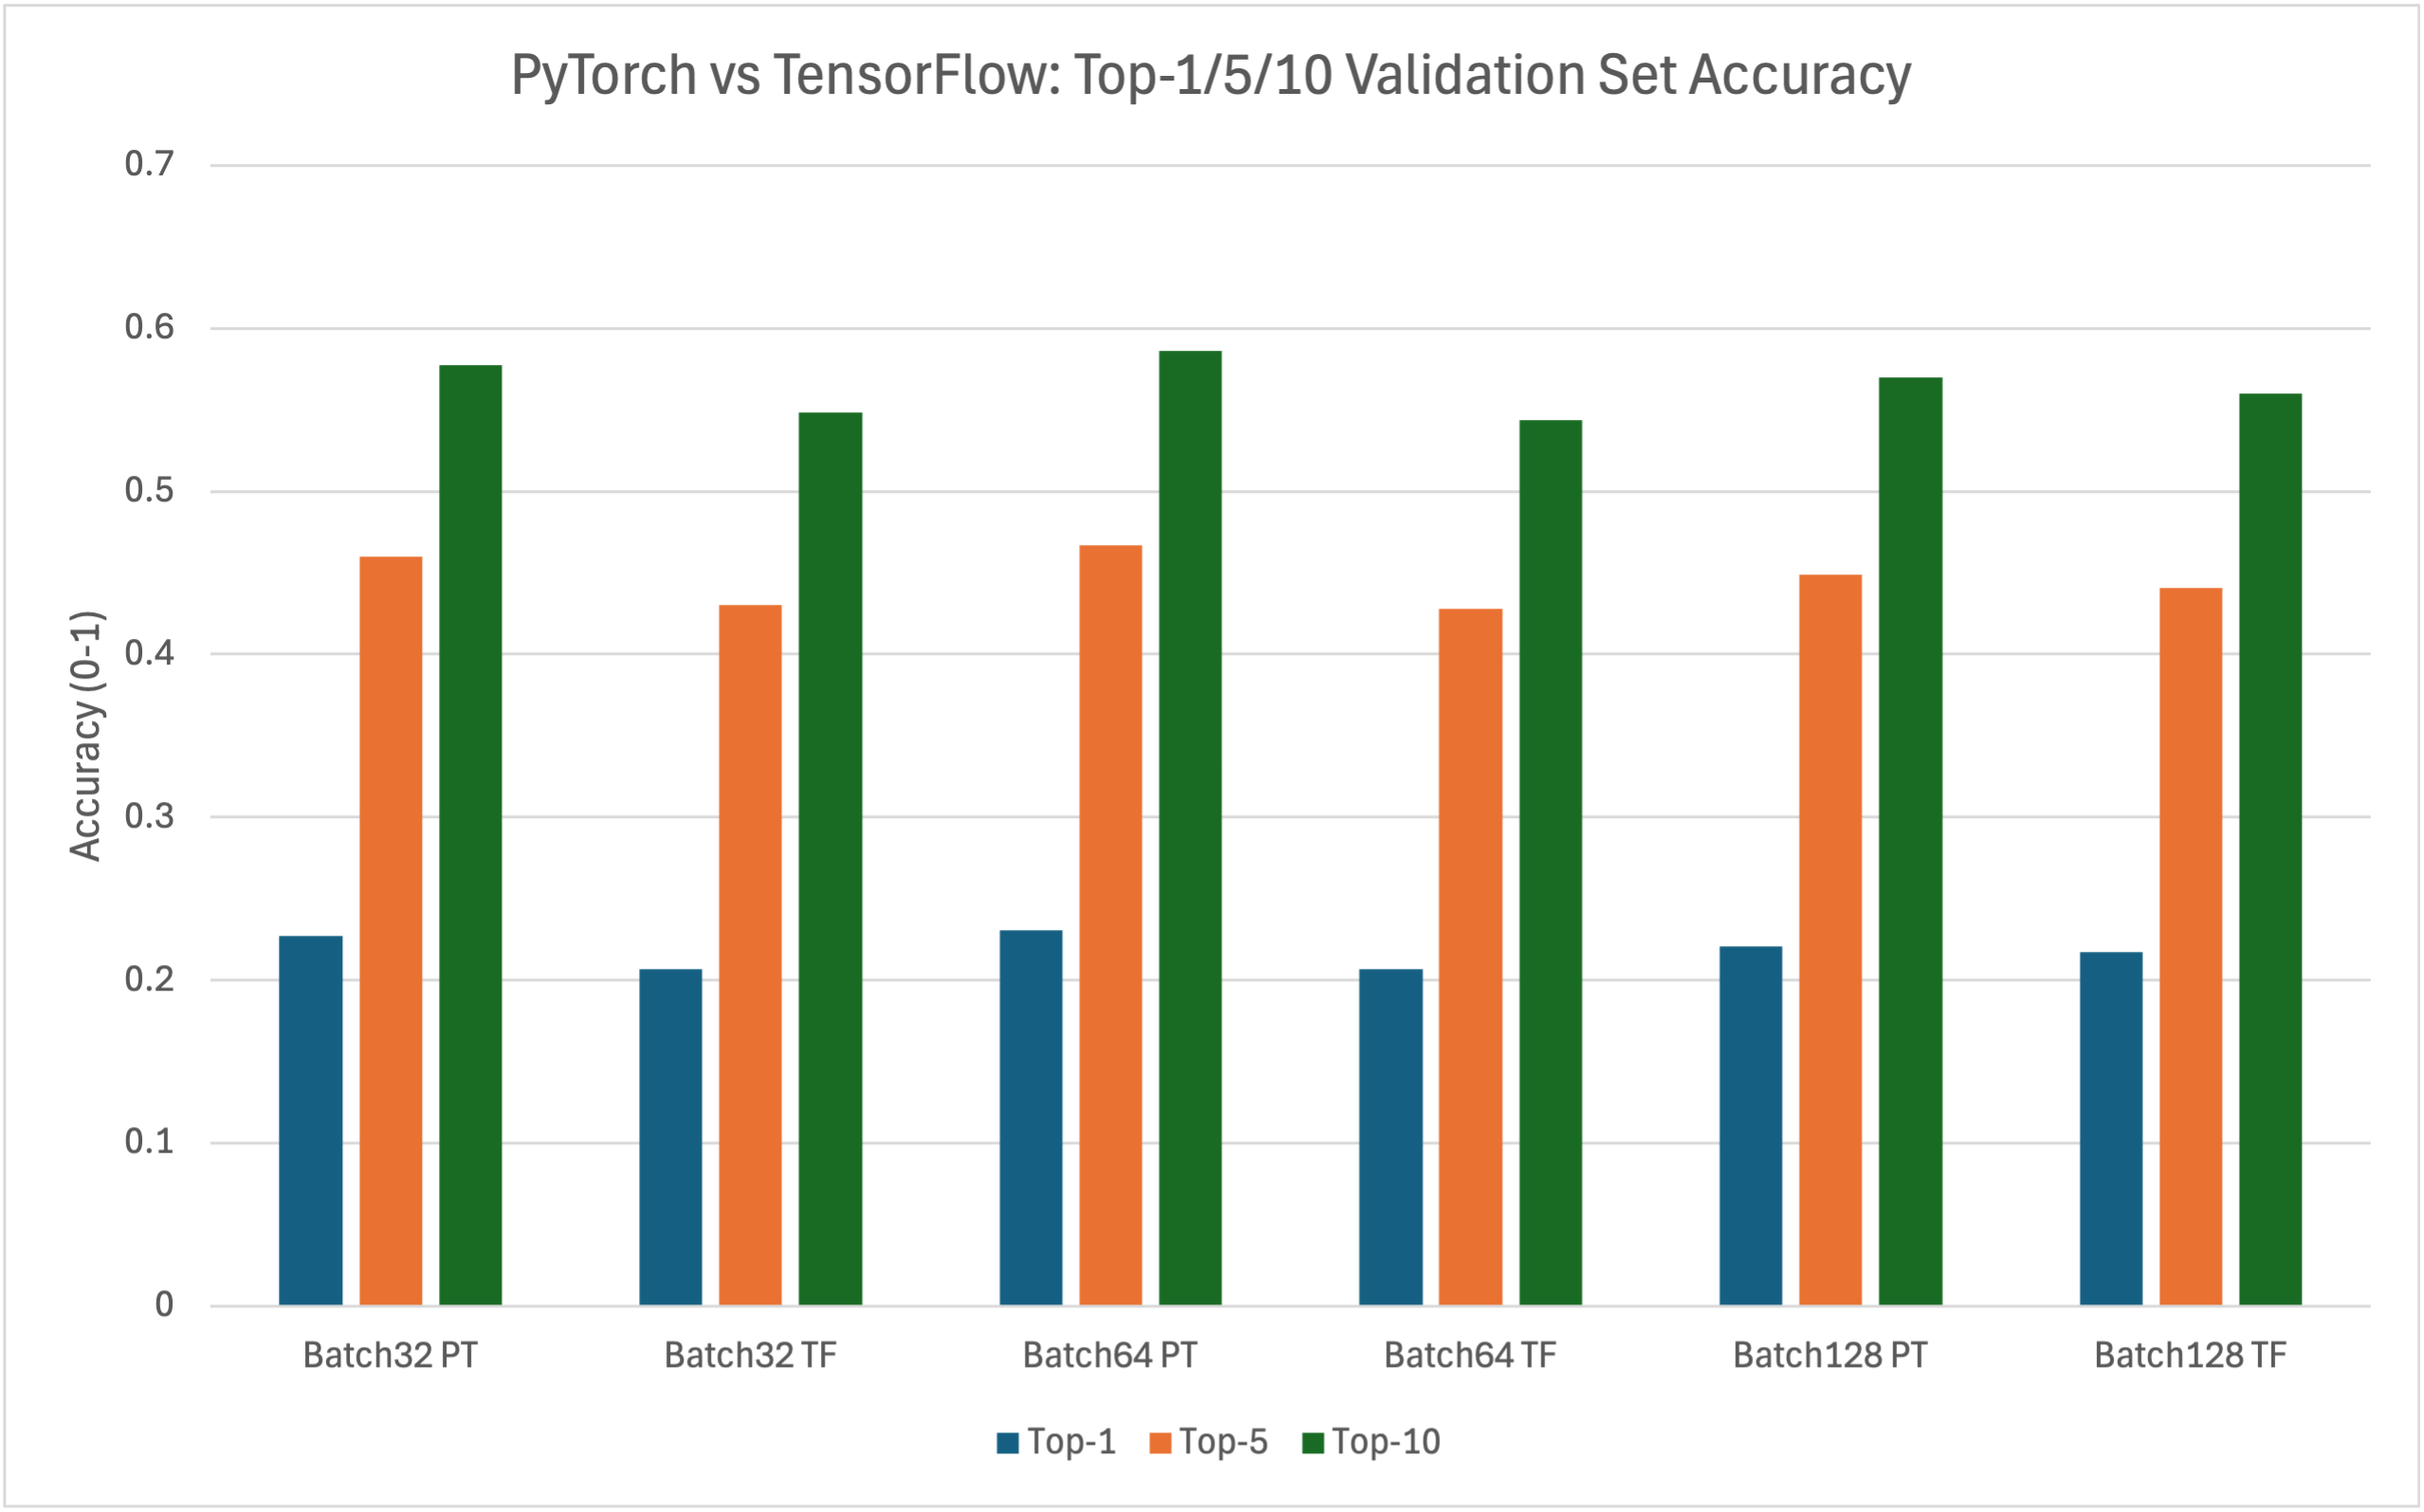
\includegraphics[width=1.0\linewidth]{Figures/Batch_Comp.png}
    \caption{\textit{Validation accuracy across batch sizes}}
    \label{fig:batchacc}
\end{figure}

Interestingly, training across a variable number of epochs with a fixed batch size of 32, we saw much worse accuracy across the board with PyTorch, sometimes over 50\% lower in a few cases. The data we collected across epochs is presented in \autoref{fig:epochacc}.

\begin{figure}[ht]
    \centering
    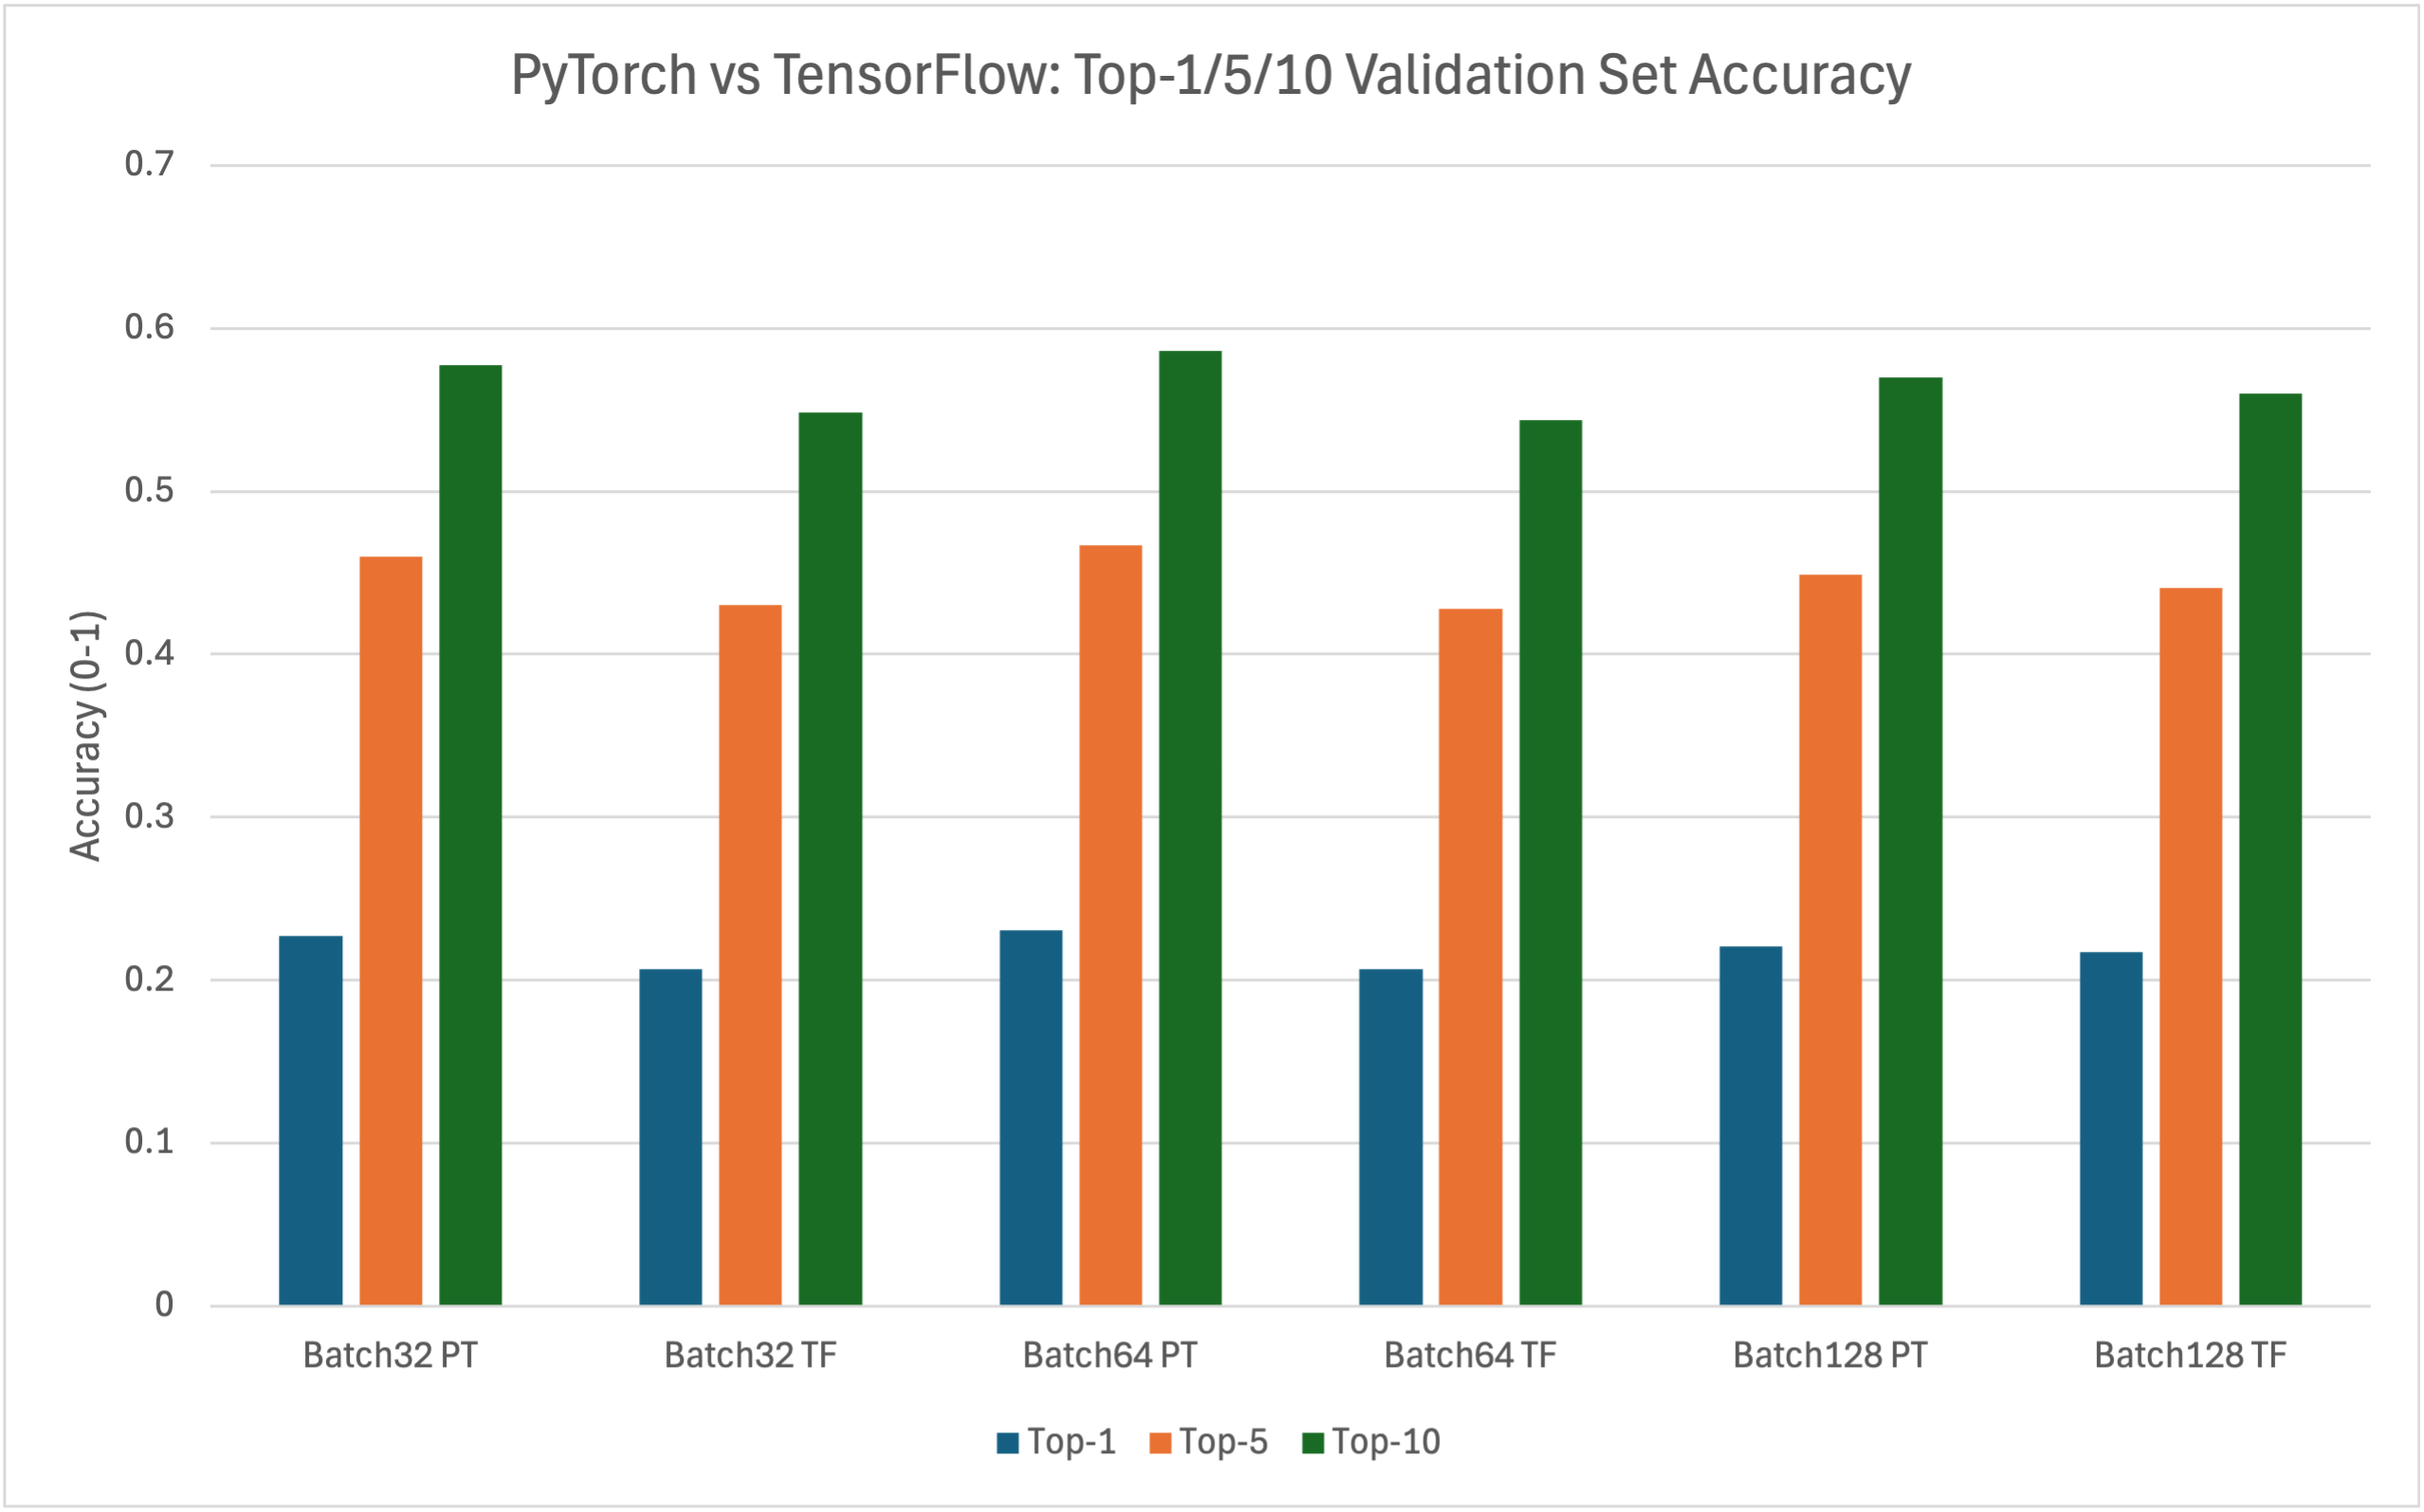
\includegraphics[width=1.0\linewidth]{Figures/Batch_Comp.png}
    \caption{\textit{Validation accuracy across epoch sizes}}
    \label{fig:epochacc}
\end{figure}

\subsubsection{Performance and Acceleration}
Both frameworks have comparable hardware acceleration support, supporting both Metal (for working with Apple devices)~\cite{tfmetal, ptmetal} as well as CUDA acceleration. PyTorch also appears to support \textit{ROCm}~\cite{ptrocm} for compute acceleration on platforms using AMD GPUs.

Before we present performance results, it's important to note that we encountered some significant struggles that we were not able to overcome when it came to running the TensorFlow environment on the same hardware that was used to benchmark PyTorch. We will discuss this challenge more in \autoref{challenges}. For this reason, the following figures will not represent a direct comparison of the two frameworks, but rather a comparison of PyTorch running on our personal machine (see \autoref{tools}) and TensorFlow running on the pre-allocated portion of the NVIDIA A40 datacenter GPU. It is reasonable to expect that TensorFlow would see some performance improvement if run on a full GPU rather than a slice.

With that disclaimer in mind, our apples-to-oranges comparison saw TensorFlow lose out significantly to PyTorch in terms of training time. \autoref{fig:batchtime} provides a graphical comparison of the results. Across batch sizes at a fixed number of 20 epochs, we saw a 30-32\% decrease in training times when using PyTorch over TensorFlow.

\begin{figure}[ht]
    \centering
    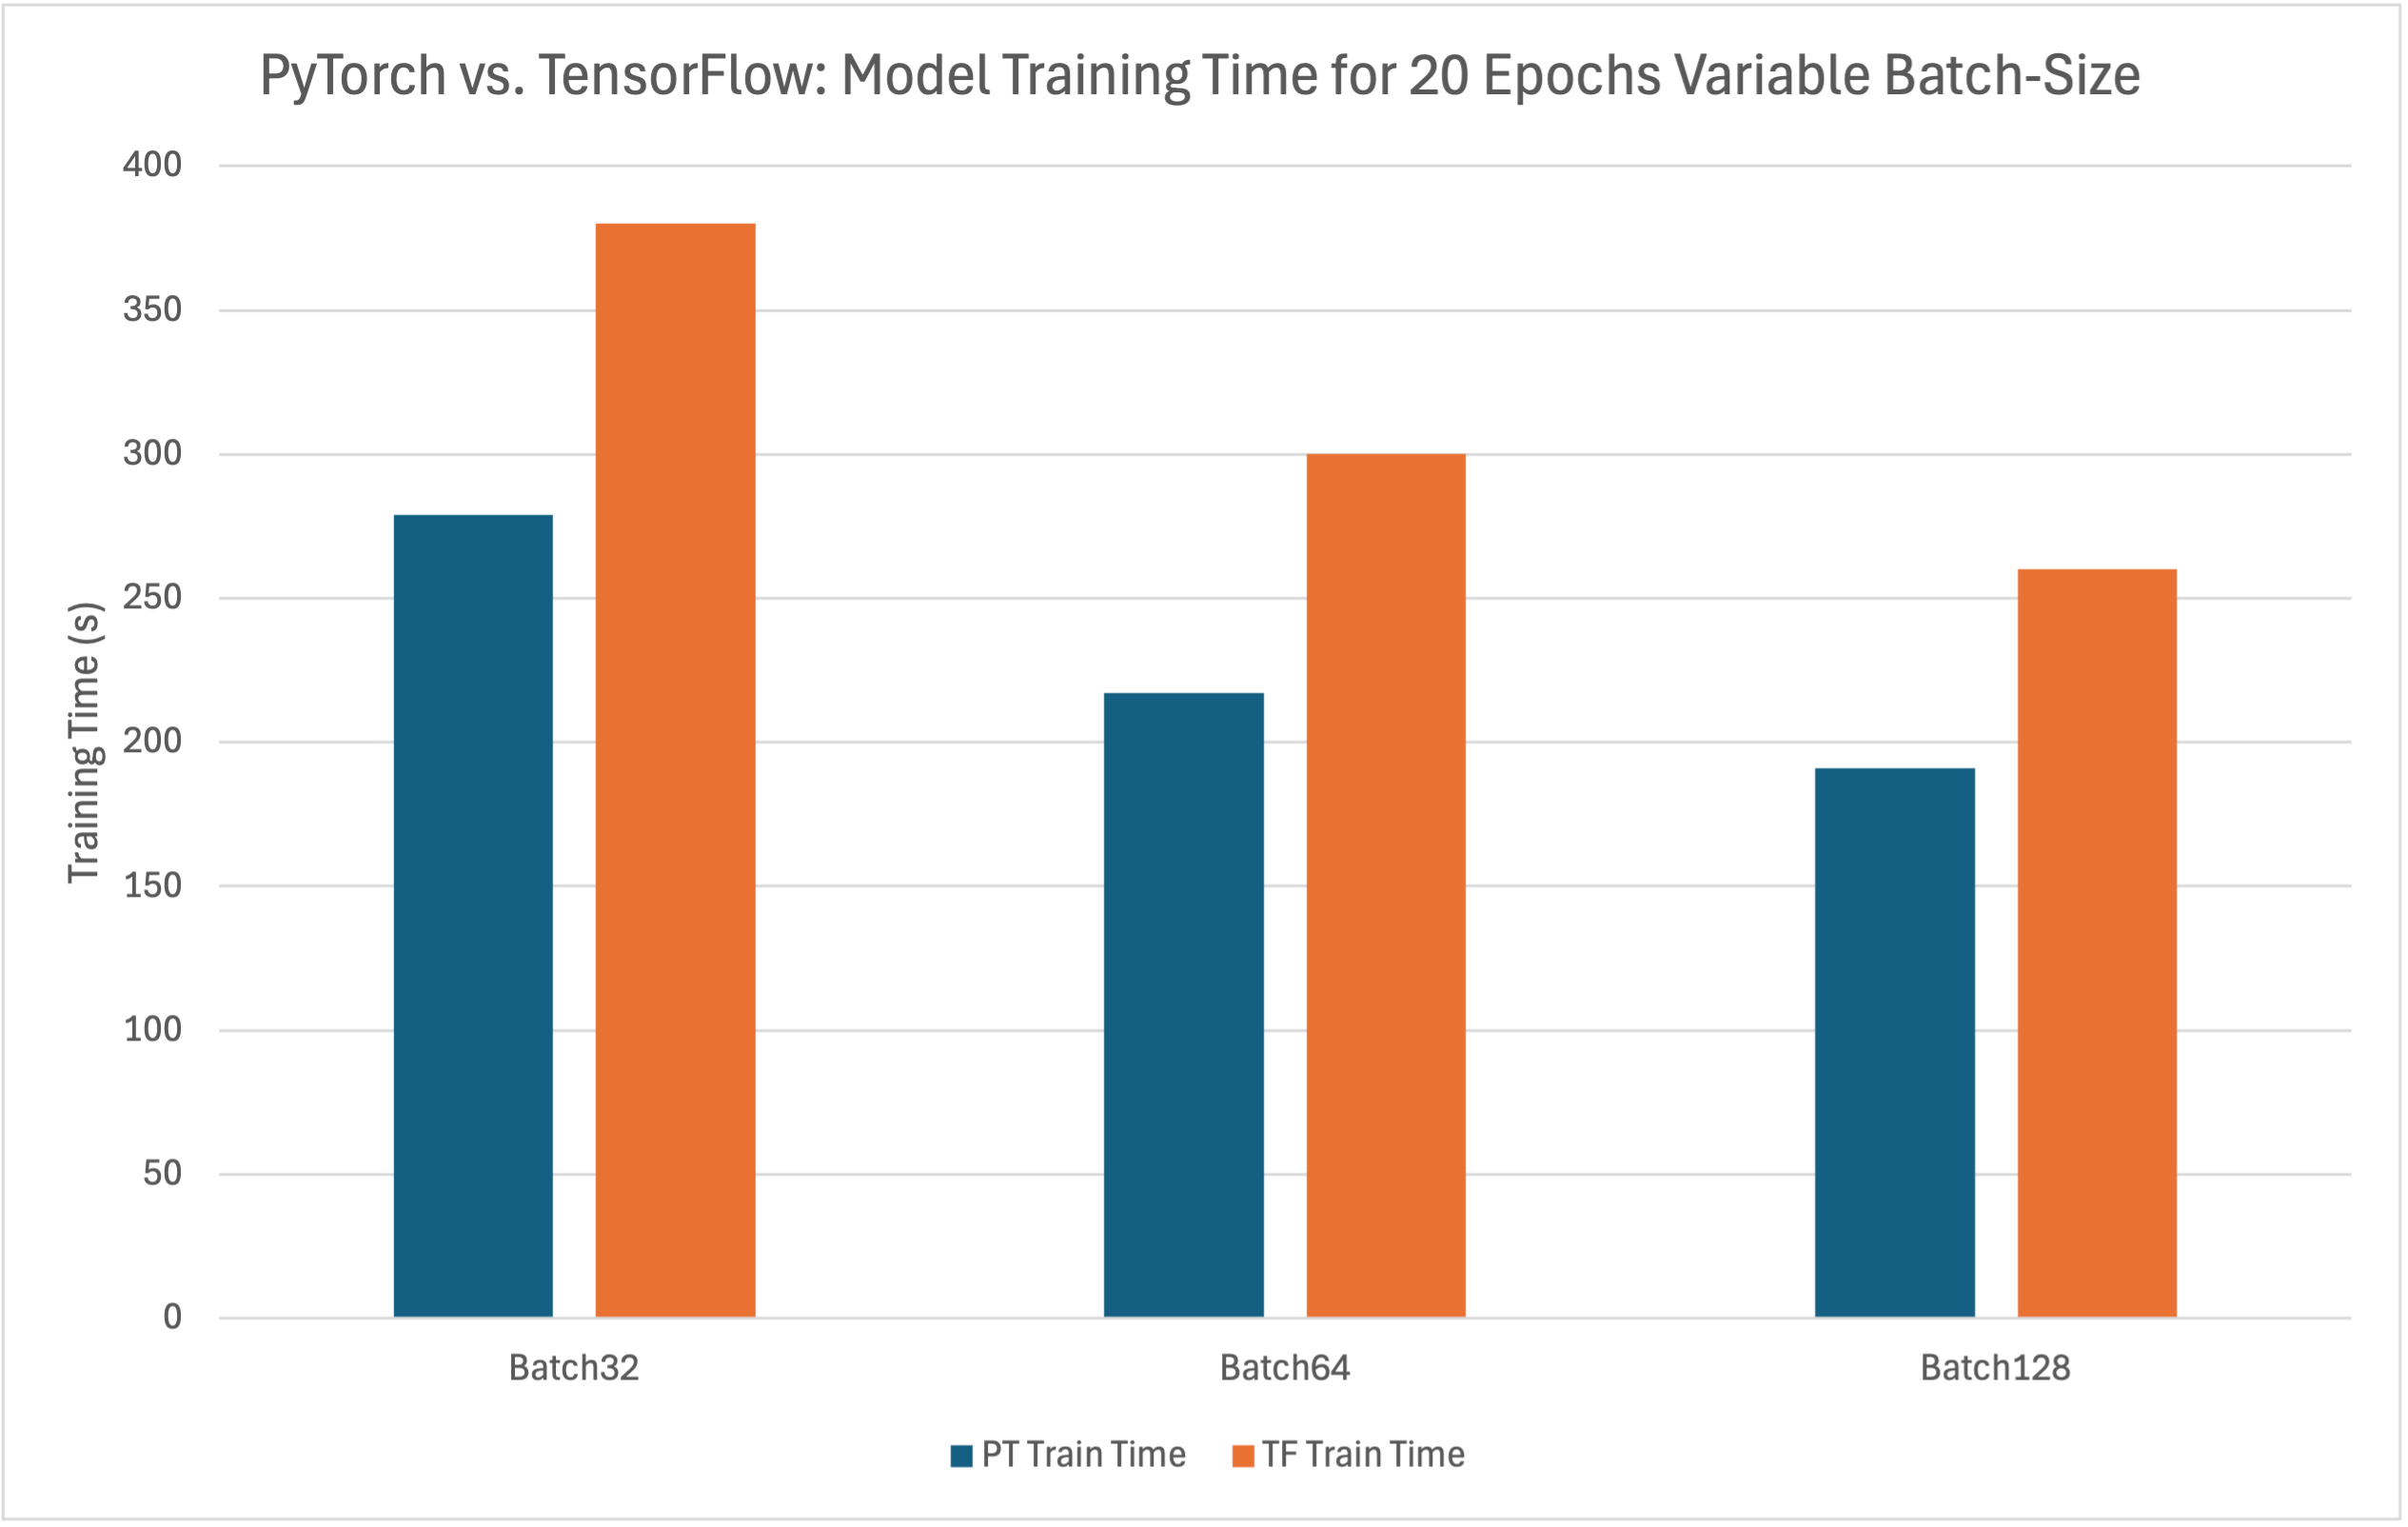
\includegraphics[width=1.0\linewidth]{Figures/batch_time.png}
    \caption{\textit{Time to train the model for 20 epochs across 32, 64, and 128 batch sizes}}
    \label{fig:batchtime}
\end{figure}

Comparing training times across 3, 10, and 100 epochs at a fixed batch size of 32, we saw an even greater improvement, from around 50 percent at the low end and 68\% at the largest number of epochs.

\begin{figure}[ht]
    \centering
    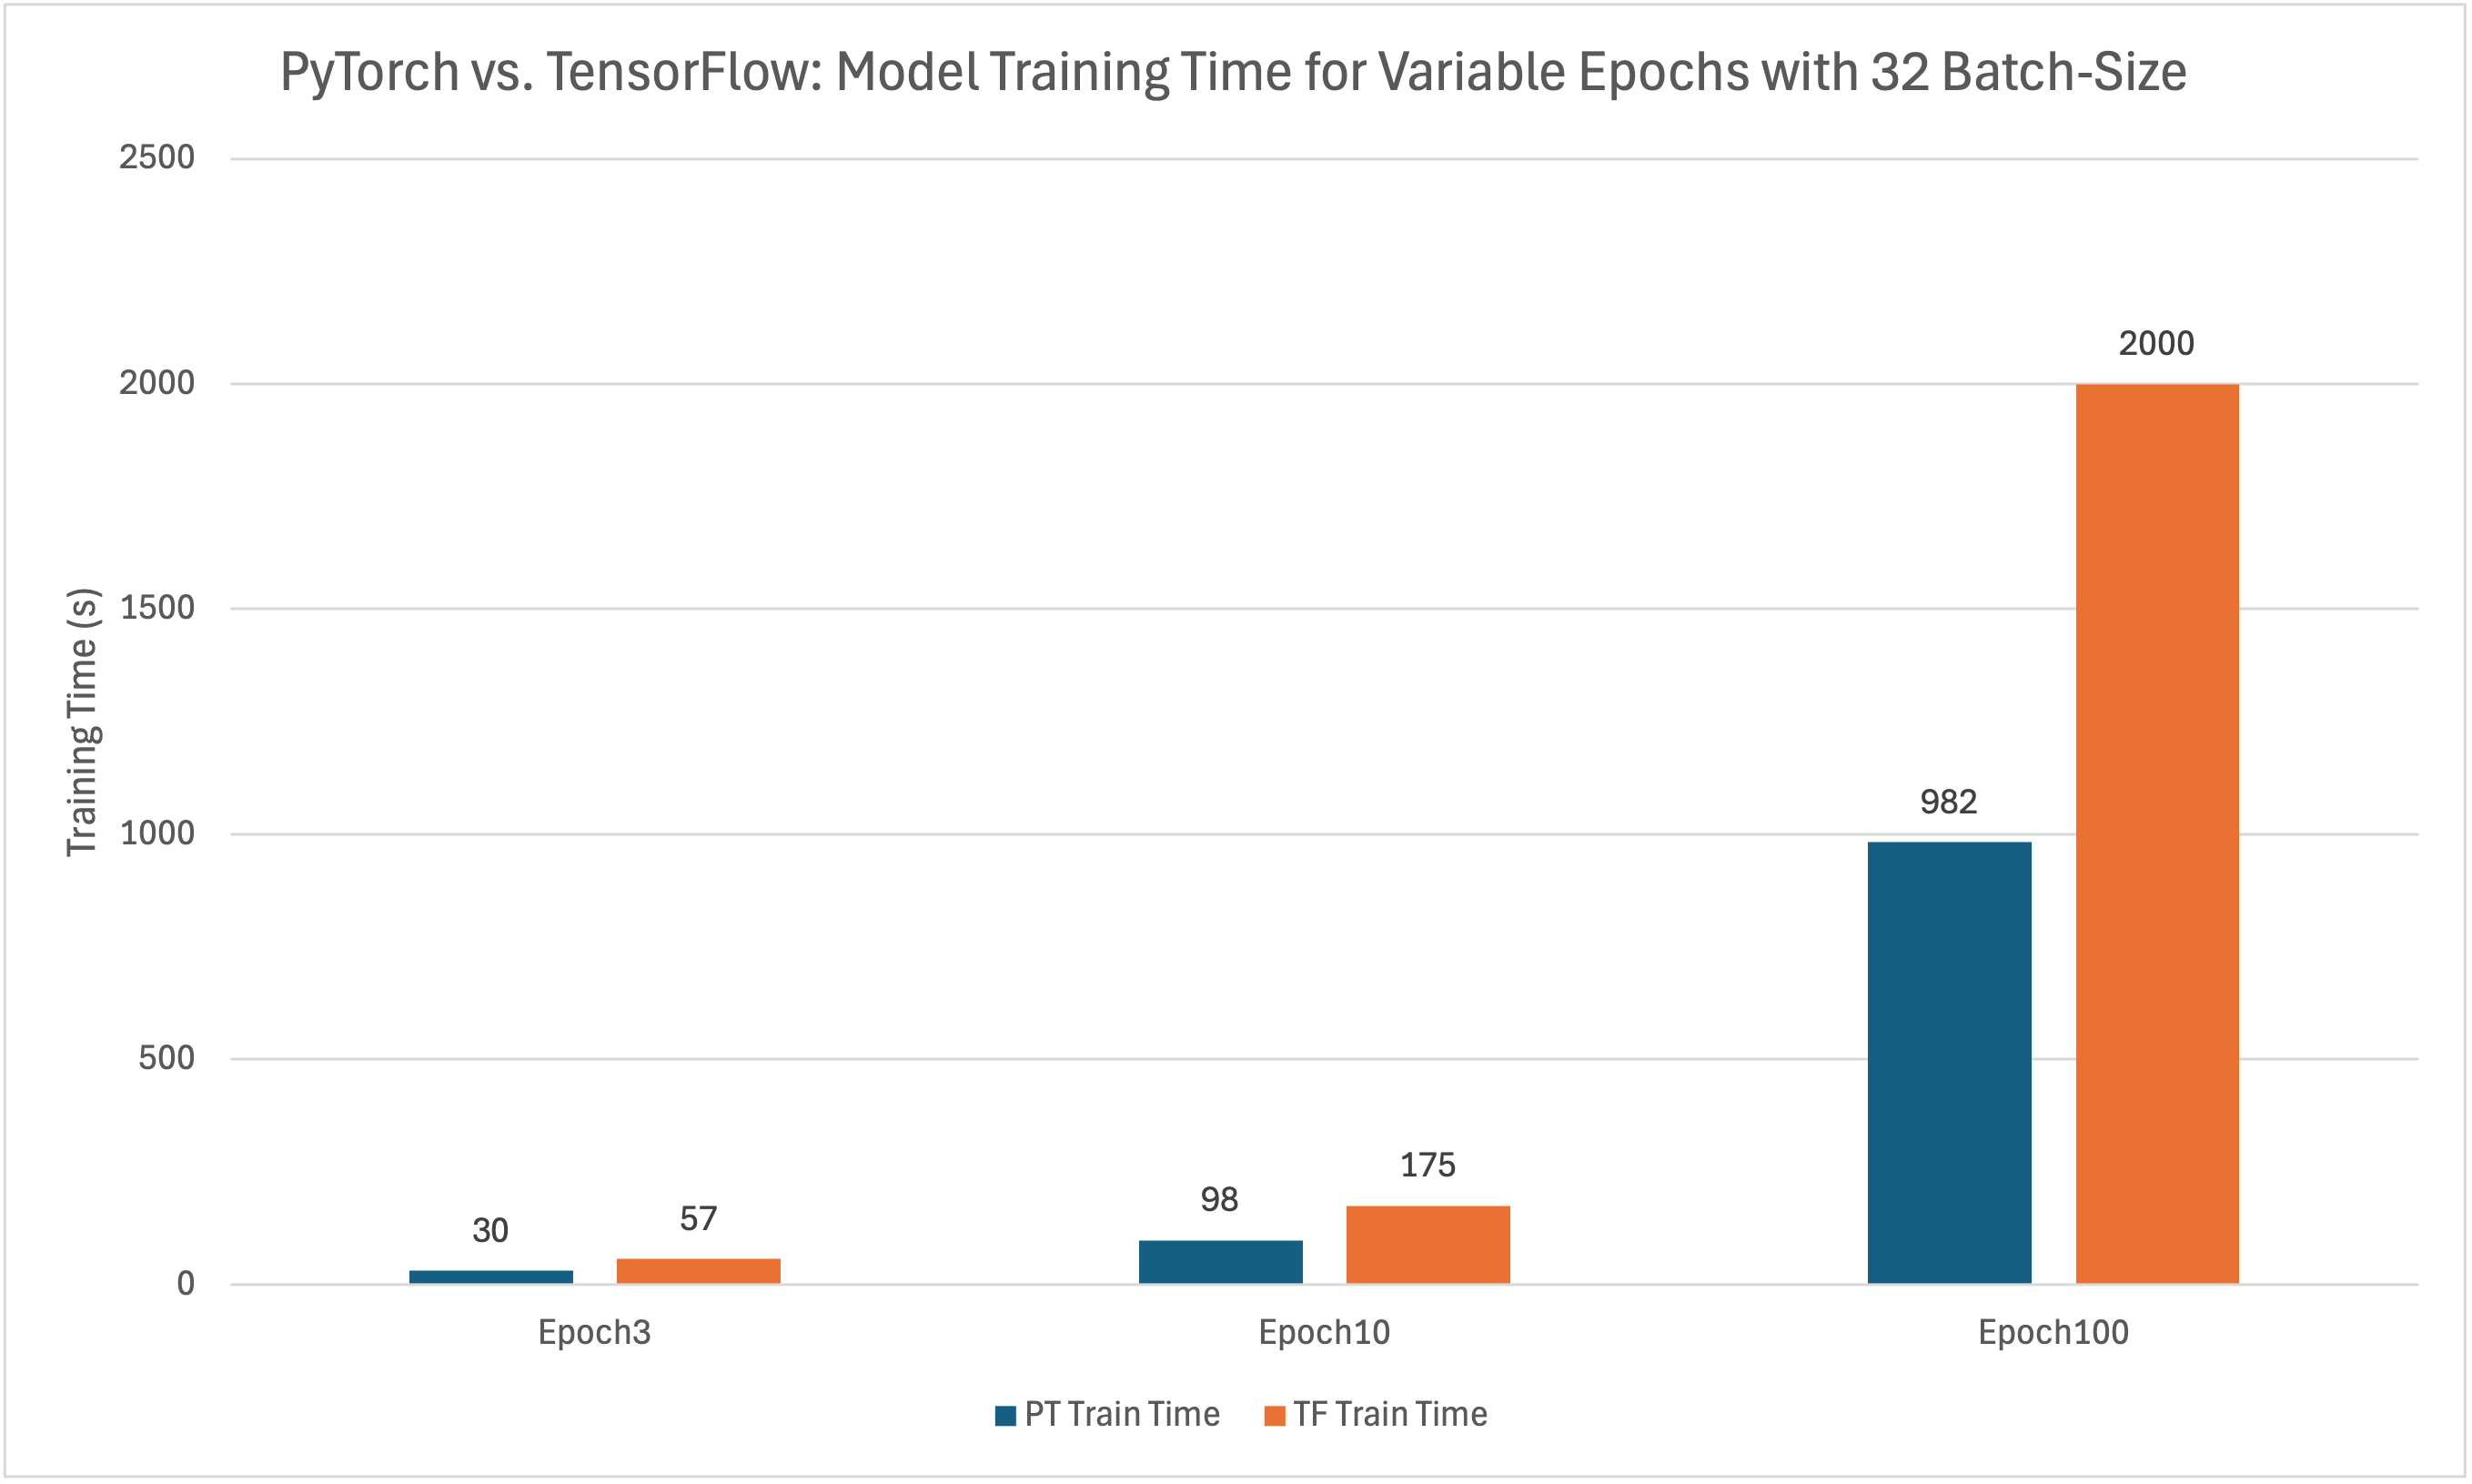
\includegraphics[width=1.0\linewidth]{Figures/epoch_time.png}
    \caption{\textit{Time to train the model for 3, 10, and 100 epochs at a batch size of 32}}
    \label{fig:epochtime}
\end{figure}


\subsubsection{Suitability of Frameworks to Device Types}
Machine learning can be applied to a variety of different situations and devices. Comparing the two frameworks, we believe PyTorch is currently more suited to high-power enthusiast and datacenter hardware. During model training, we were able to achieve about 95\% utilization of the RTX 3090's core while consuming \~6GB of VRAM and 300W of power with the whole model and dataset loaded in. This gave us great performance, but is obviously not suitable for low-power edge applications like a mobile phone. While there \textit{does} exist a library called ExecuTorch, aimed at running PyTorch models on edge devices~\cite{executorch}, it does not currently support training models. On the other hand, TensorFlow Lite has full support for training models on any device that supports it~\cite{tflite}. TensorFlow also has dedicated hardware for edge applications, such as the Pixel Neural Core~\cite{pixel}, further cementing it as the framework of choice for such scenarios.

\subsection{Deliverable 2: Lab 1 Revised Manual and Student Template}
In addition to the updated Lab 1 notebook with our PyTorch implementation, we are also providing a modified Lab 1 manual that changes several sections to be in accordance with how they are now performed in PyTorch. To go along with the manual, we've provided a "template" Lab 1 notebook that has sections removed according to what should be completed by the student.

\section{Documentation}

As part of our deliverables, we included a revised lab 1 manual to document the modifications we made, the tools and code we provide, and the instructions for future students to complete the lab in the case this were to be used as an alternate to lab 1. Additional key specifications about our project are included here.

\newpage
\subsection{Project Contents}
\dirtree{%
.1 /.
.2 README.md - Instructions, documentation, and resources.
.2 /pytorch - Lab 1 with PyTorch.
.3 /img\_data - Input image binaries.
.3 /model\_data - Intermediate layer weights binaries.
.3 /log\_data - PyTorch Profiler performance traces.
.3 /trained\_models - Additional models trained from the notebook.
.3 /tutorial - PyTorch tutorial notebooks for getting started.
.3 GPU\_Dataset.py - Class to pre-load dataset when using a GPU.
.3 tinyimagenet\_model.pt - The toy model to run inference with.
.3 TinyImageNetModel.py - Class to architect the toy model.
.3 Lab1\_PyTorch.ipynb - Lab notebook.
.3 Lab1\_PyTorch\_Template.ipynb - Lab notebook template for students to complete and submit.
.3 requirements.txt - PyTorch and related packages.
.2 /tensorflow  - Lab 1 with TensorFlow.
.3 /img\_data - Input image binaries.
.3 /model\_data - Intermediate layer weights binaries.
.3 /log\_data - Tensorboard performance traces.
.3 /tutorial - TensorFlow tutorial notebooks for getting started.
.3 CNN\_TinyImageNet\_2.h5 - The toy model to run inference with.
.3 Lab1\_TF.ipynb - Lab notebook.
.3 requirements.txt - TensorFlow and related packages.
}

\subsection{Project Tools} \label{tools}
We used VS Code for development and a local workstation for accelerated training times. The specs include an AMD Ryzen 9 5900X CPU and a NVIDIA RTX 3090 GPU.

\subsection{Installation and Use}
The project requires a few different dependencies to be satisfied before the user is able to run the Jupyter notebook. These dependencies can be found in \verb|/pytorch/requirements.txt|. After the user has installed Python >= 3.9 and (optionally) created a \verb|venv| and activated it, they may run the following command to automatically install the necessary packages as they were set up when we completed the project: \verb|pip install -r ./pytorch/requirements.txt|. 

If the user wishes to utilize CUDA acceleration, they will need to either install the appropriate CUDA drivers on their machine or be running the Jupyter notebook while remotely connected to a machine that already does. The same holds true with AMD devices. Metal support for Apple devices is already baked in and requires no additional user action. More details can be found in the project's README.

\section{Challenges Faced} \label{challenges}
There were a few challenges faced over the course of the project. The team was able to adhere to the project timeline fairly well, with a few delays related to technical issues. One of the smaller challenges was getting the CUDA development environment setup. This involved installing the needed CUDA packages and finding ways to monitor GPU usage. Once using the CUDA environment, the team had to spend time going back through the code in order to make sure that all of our data was stored on the correct devices at a given time. This involved adding \verb|.to(device)| and \verb|.cpu()| to different tensors when they were needed on the GPU or CPU. The team was also able to optimize some of the transfers this way, by doing all of the transfers before iterating through the data as opposed to transferring the data in the loop each time. The biggest challenge faced however was getting the training to work correctly. There were many issues getting the loss to back propagate correctly and update all of the variables in the training. This would cause the loss to stay at a relatively constant value on each iteration. This challenge took the team the most time to fix on the PyTorch side and was ultimately solved. On the TensorFlow side of the project, the largest challenge we faced was replicating the Python lab environment. The team spent multiple hours trying to setup a python virtual that matched the lab computers. This involved using conda, pyenv, and attempting to match the versions of all of the required packages. Ultimately, we were still not able to find a solution that resulted in a functioning Python environment with the necessary packages to allow us to run the TensorFlow notebook.

\subsection{Model Setup and Training Challenges}
Our group also faced a set of difficulties that tied into model structure and training. Initially, the team had structured the model identically to how it was set up in TensorFlow, and this didn't present itself as an issue until we had moved into the model training portion of the lab. Upon attempting to train the model, the team discovered that the loss per batch essentially stayed constant at \~5.28. After some research, the team discovered that this could be due to the fact that the \verb|CrossEntropyLoss()| function expects the raw output of the model, not classifications, which due to the Softmax layer being present, was not what we were giving the loss function. With this layer removed from our model definition, we reran our training loop and still saw no change. We were initially under the assumption that we had somehow improperly coded our training loop and that the loss and parameter updates were not being applied, but our code was very similar to the official examples and recommendations that were provided. Ultimately, the issue ended up being related to the default initialization of the model. We had assumed that the default initialization values would have been sufficient, but after using a \textit{Kaiming Uniform} initialization, we were finally able to see our loss per epoch trend downward.

{\footnotesize\bibliographystyle{acm}
\bibliography{report}}

\end{document}
